% !TEX root =  main.tex
\section{Introduction}\label{sec:intro}
Smart contracts are programs running on top of blockchain platforms such as
Bitcoin~\cite{bitcoin} and Ethereum~\cite{ethereum}.  They interact with each
other to perform effective financial transactions in a distributed system
without the intervention from trusted third parties (e.g., banks). A smart
contract is written in a high-level programming language (e.g.,
Solidity~\cite{solidity}), and it is typically comprised of a unique address,
persistent storage holding a certain amount of cryptocurrency (i.e., Ether in
Ethereum), and a set of functions that manipulate the persistent storage to
fulfill credible transactions without trusted parties. For contract-to-contract
interaction, some functions are public and callable by other contracts. Thanks
to the expressiveness afforded by the high-level programming languages and the
security guarantees from the underlying consensus protocol, smart contracts have
shown many attractive use cases, and their number has skyrocketed, with over 45
million~\cite{etherscan} instances covering financial products, online gaming,
real estate~\cite{case1}, shipping, and logistics~\cite{case2}.

Because all smart contracts deployed on a blockchain are freely accessible
through their public methods, any functional bugs or vulnerabilities inside the
contracts can lead to disastrous losses, as demonstrated by recent
attacks~\cite{attack1,attack2,attack3,attack4}. For instance, the code (simplified) in
Figure~\ref{fig:motivate} illustrates the notorious \reentrancy attack~\cite{attack1}. When the
victim program (3) issues a money transaction
to the attacker (2), it implicitly triggers the attacker's callback method, 
which invokes the victim's method (i.e., \texttt{withdraw}) again to make
another transaction without updating the victim's balance. The attack maliciously extracted tokens
from the victim and led to
a financial loss of \$150M in 2016. To make things worse, smart contracts are
immutable---once they are deployed, fixing their bugs is extremely difficult due
to the design of the consensus protocol.\looseness=-1

% Improving robustness of smart contracts is thus a pressing practical problem.
% It is also an active area of research, with several contract analysis 
% tools~\cite{oyente,securify,contractfuzzer,madmax,zeus,teether} developed in the
% past few years. However, these tools either soundly overapproximate the
% execution of smart contracts and report warnings~\cite{securify,madmax} that
% cannot be exploited in reality, or they precisely
% enumerate~\cite{teether,contractfuzzer,oyente} \emph{concrete traces} of smart
% contracts, so cannot scale their analyses to large programs.

% \todo{Improving robustness of smart contracts is thus a pressing practical problem. Unsurprisingly,
% a complex vulnerability like \reentrancy typically involves interactions between multiple contracts, 
% which requires an analyzer to \emph{precisely} model the inter-contracts communication 
% and reason about the execution in a \emph{precise} and \emph{scalable} way.
% But existing tools either soundly overapproximate the
% execution of smart contracts and report warnings~\cite{securify,madmax} that
% cannot be exploited in reality, or they precisely
% enumerate~\cite{teether,contractfuzzer,oyente} \emph{concrete traces} of smart
% contracts, so cannot scale their analyses to large programs.}

Improving robustness of smart contracts is thus a pressing practical problem. Unsurprisingly,
 a complex vulnerability like \reentrancy typically involves interactions between multiple contracts, 
 which requires an analyzer to model the inter-contracts communication 
 and reason about the execution in a \emph{precise} and \emph{scalable} way.
 But existing tools either aggressively \emph{overapproximate} the execution a smart contract and report warnings~\cite{securify,madmax} that do not correspond to 
 feasible paths and therefore cannot be exploited, or they precisely
 enumerate~\cite{teether,contractfuzzer,oyente} \emph{concrete traces} of a smart
 contract, so cannot scale to large programs with many paths.

% As a result, it is vital to develop precise and scalable analysis techniques to 
% ensure the safety and robustness of smart contracts, and identify potential 
% \emph{malicious attacks} before deployment. But precise analysis is especially 
% challenging in this setting because it depends on precisely modeling a 
% contract's interactions with other parties on the blockchain. 
% Without a precise  interaction model,  blindly applying traditional bug finding and 
% verification techniques to smart contracts leads to a high false positive rate
% and vulnerabilities that are infeasible to exploit. 

% \begin{figure}
%     % \centering
%     \begin{subfigure}[b]{0.4\textwidth}
%     \begin{lstlisting}
% contract Victim {
%   mapping (address => uint) public balances;

%   function withdraw() public {
%     uint amount = balances[msg.sender];
%     //call withdraw again
%     msg.sender.call.value(amount)(); 
%     balances[msg.sender] = 0;
%   }
% }
%     \end{lstlisting}
%     \caption{The Vulnerable Program}
%       \label{fig:dao-vic}
%     \end{subfigure} \\
%     \begin{subfigure}[b]{0.4\textwidth}
%     \begin{lstlisting}      
%   contract Attacker {
%     ...
%     function () payable {
%       Victim v;
%       v.withdraw();
%     }
%   }
% \end{lstlisting}
%     \caption{The Attack Program}
%       \label{fig:dao-attack}
%     \end{subfigure}
% \caption{Reentrancy Attack \label{fig:intro-example}}
% \end{figure}
% \begin{figure}
%   \centering
%   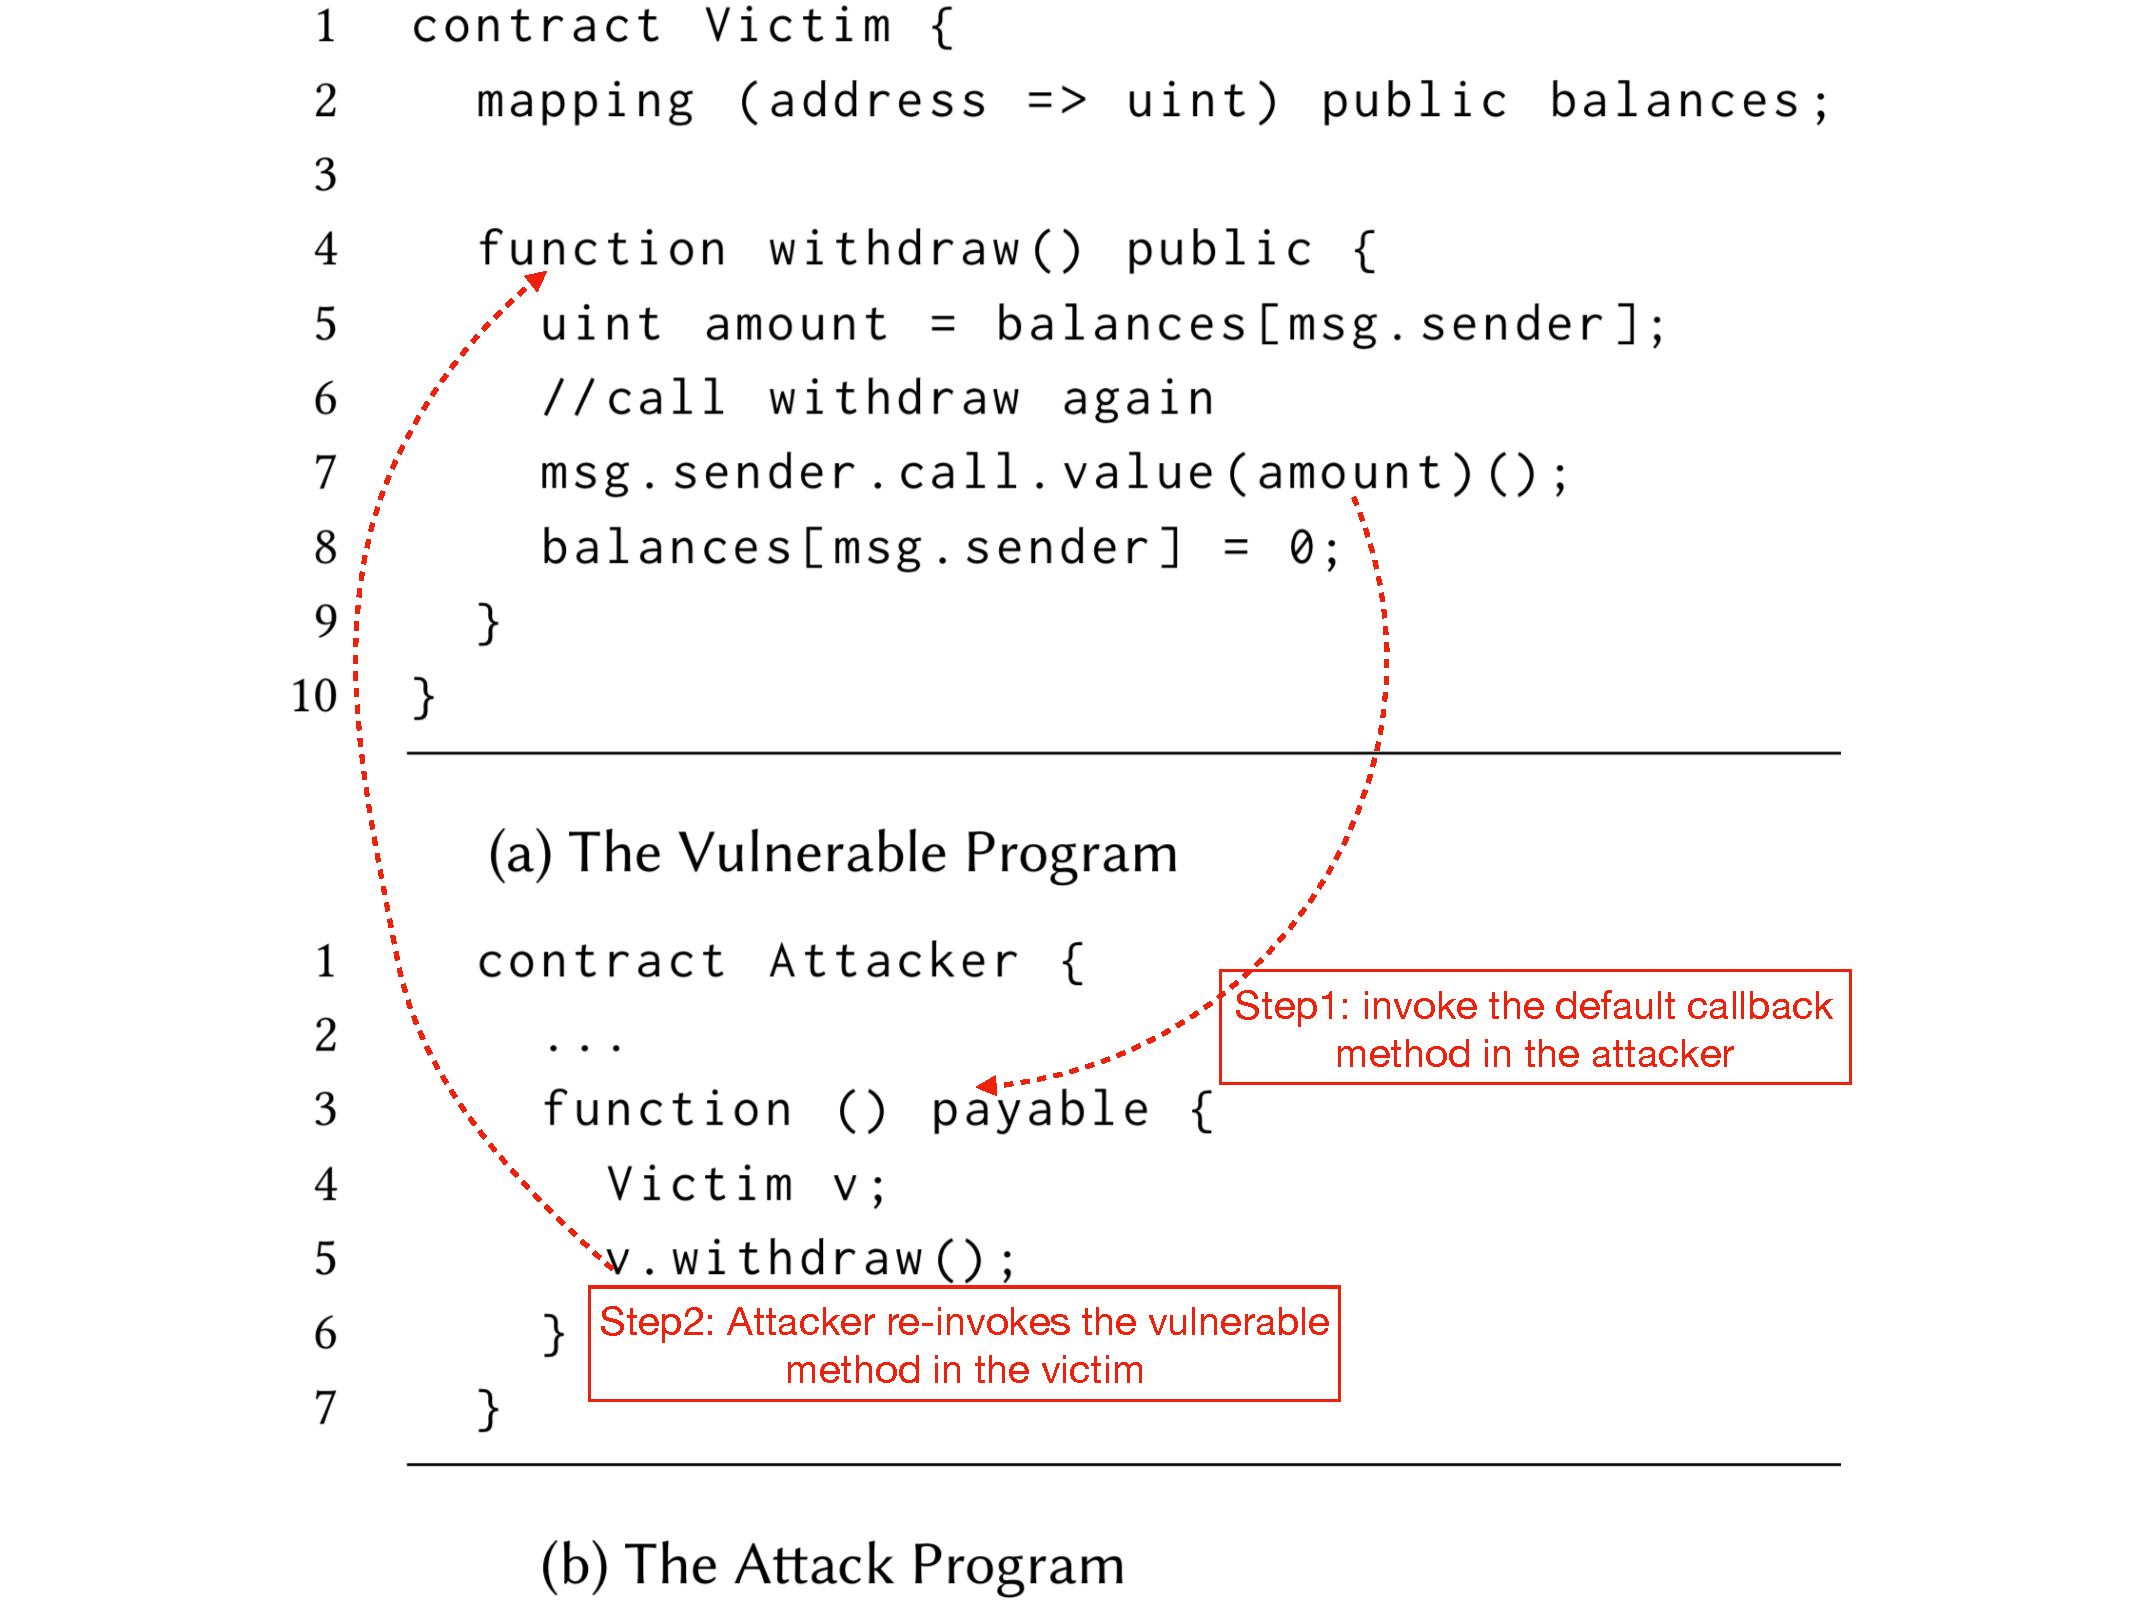
\includegraphics[scale=0.26]{reentracy.pdf}
% \caption{Reentrancy Attack \label{fig:intro-example}}
% \label{fig:batchcode}
% \end{figure}



% This paper presents \toolname, a tool that uses \emph{program synthesis} to
% automatically generate adversarial smart contracts (i.e., attack programs),
% which exploit common vulnerabilities in victim contracts. \todo{Our design choice is based on two key insights. First, an effective way to test the security properties of a smart contract is to construct \emph{real} exploits triggered by attack contracts, which faithfully simulates the untrusted execution environment on blockchains. Second, a security analyst can easily initialize boilerplate code (e.g., constructor of the victim with its address) for the basic communication channel between the attack and victim contracts, and then leverage constraint solvers to \emph{synthesize} an attack contract by efficiently exploring the search space defined by the victim's public interface.}
This paper presents \toolname, a new point in the design space of smart contract analysis tools that achieves an effective trade-off among expressiveness, precision, and scalability. \toolname provides the security analyst with a query language for expressing \emph{vulnerability patterns} 
that can be exploited in an attack, as well as an automatic engine for \emph{synthesizing} an attack program (if one exists) that exploits the given vulnerability. Our key insight is based on the observation that an attacker typically exploits the vulnerability by making a sequence of transitions (calls over public methods of the victim), in which storage states are preserved across different transitions. As shown in Section~\ref{sec:vul}, because most types of vulnerabilities can be overapproximated through assertions over storage variables, this insight motivates an effective summary-based symbolic evaluation technique where the summary of a method soundly models its side-effect over storage variables, which dramatically reduces the number of instructions that \toolname has to re-evaluate symbolically. As a result, \toolname is able to scale reasoning with better precision to large contracts that are out of reach of existing symbolic execution~\cite{teether,oyente} and fuzzing~\cite{contractfuzzer} tools. 
% Our engine employs a novel summary-based symbolic evaluation technique to scale precise reasoning to large contracts 
% that are out of reach of existing symbolic execution~\cite{teether,oyente} and fuzzing~\cite{contractfuzzer} tools. 
Furthermore, previous summarization techniques~\cite{AnandGT08,Godefroid07} rely on symbolic execution and 
can therefore lead to summaries that are exponential in program size. 
Our technique relies on Rosette~\cite{rosette}, a hybrid symbolic evaluator that combines symbolic execution and bounded model checking, 
to compute compact (i.e., polynomially-sized) and precise (i.e., encoding all feasible bounded paths) summaries at the procedure level. 
%In particular, the size of the summary is polynomial in the size of the procedure, and the summary precisely encodes 
%the meaning of {all} (bounded) paths through that procedure. 
Using these summaries, \toolname can perform precise all-paths analysis of 
 a given contract
while symbolically executing significantly fewer paths than Rosette alone.\looseness=-1

To use our tool, a
security analyst expresses a target vulnerability query (e.g., the reentrancy
vulnerability) as a declarative specification.  
\toolname then \emph{synthesizes} an attack program that exploits the victim's public
interface to satisfy the vulnerability query. Given this problem, a naive
approach is to enumerate all possible candidate programs and then symbolically
evaluate each of them to check if it satisfies the query. While precise, the
naive approach fails to scale to realistic contracts. 
%To tackle this challenge,
%we employ a novel \emph{summary-based symbolic evaluation}, which enables
%\toolname to both find real attacks and scale to large programs. 
\begin{figure}
  \centering
  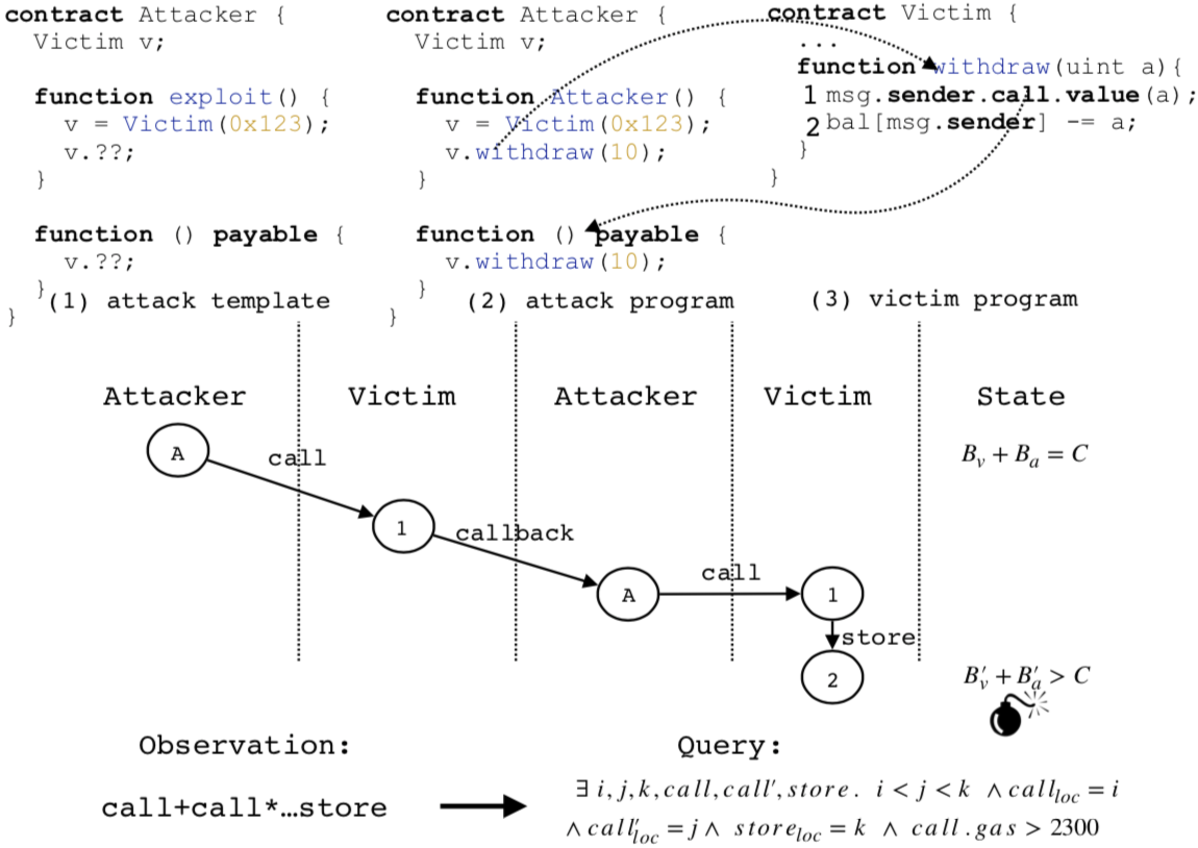
\includegraphics[scale=0.40]{motivate.pdf}
\caption{Sample contracts to show the Reentrancy attack.}
\label{fig:motivate}
\end{figure}
% Fig~\ref{fig:overview} shows an overview of our approach. Given the public
% methods provided by the Application Binary Interface (ABI) of a smart contract,
% our system first \emph{symbolically} evaluates each method and generates a
% summary that soundly records the method's side-effects on the storage as well as
% other global state of the Blockchain. 
Even with summarization, the search space
is still too large for brute-force enumeration. To address this issue, we
partition the search space by case splitting on the range of symbolic variables,
which allows us to simultaneously explore multiple attack programs using Rosette's 
SMT-based symbolic evaluation engine~\cite{rosette}. 
% \toolname further reduces
% the search space by pruning infeasible candidates early, using their symbolic encoding to 
% quickly check for the absence of potentially exploitable paths. After that, our tool symbolically evaluates each
% remaining candidate to check if any of them satisfies the vulnerability query.
% If so, the candidate is returned as a potential exploit.\looseness=-1

%  we present an efficient and precise approach for 
% reasoning about security properties of smart contracts. Given a contract under 
% test, our tool will synthesize an \emph{attack program} (i.e., adversarial smart contract) that 
% exploits a vulnerability expressed in our query language. 
% The attack program models a feasible set of interactions between 
% the contract under testing and the outside world, making our technique precise. 
% The technique is also complete within a user-provided bound on the size of the attack program.

% To use our technique for finding vulnerabilities in a contract, 
% a security analyst provides its implementation (binary or source), 
% the Contract Application Binary Interface (or just ``ABI" for short) 
% listing the contract's public methods that can be accessed by a third-party contract, 
% and a vulnerability query $\query$ in the form of first-order formula over 
% \emph{program states}. For instance, the Reentracy vulnerability in Figure~\ref{fig:intro-example} can be expressed as the
% following query: synthesize an attack program such that: 1) the program can invoke a sequence of public APIs provided by 
% the victim contract. 2) On executing the attack program, there exists a trace such that it contains 
% \emph{at least two consecutive} \texttt{calls} before a store operation. For instance, the attack program in 
% Figure~\ref{fig:dao-attack} can generate a trace like the following: \texttt{call call call store}
% which eventually leads to a DAO attack. 
%  \todo{Can we add a sentence here about the expressive power of the query language? What kinds of attacks can it capture?}

% Given these inputs, our technique iteratively enumerates \emph{sketches}~\cite{sketch-paper} of possible attack programs. 
% Each sketch $\sketch$ is composed of method calls to the public methods from the ABI, where   
% the arguments of all method calls are \emph{symbolic}.
% The technique then evaluates the sketch $\sketch$ using an off-the-shelf symbolic virtual machine~\cite{rosette}, 
% obtaining a symbolic program state $\pstate$ that encodes all reachable states 
% of $\sketch$. Since the original vulnerability query $\query$ is written in a formula over program 
% state $\pstate$, we leverage an SMT solver to check if there exists a concrete 
% interpretation $I_b$ for $\pstate$ where $\query$ holds. If the answer is yes,  
% we obtain a concrete attack program from $I_b$. Otherwise, we try other 
% candidate sketches (up to a user-specified bound on attack program size). 
% \todo{Can we add a sentence here describing the key technical novelty: is it the sketch enumeration algorithm or some other way to carefully control the search space to ensure scalability?}

We have evaluated \toolname on the entire data set ($>$25K) from
\etherscan~\cite{etherscan}, showing that our tool is expressive, efficient, and
effective. \toolname's query specification language is expressive in that it is
rich enough to encode common vulnerabilities found in the literature (such as the
Reentrancy attack~\cite{attack1}, Time manipulation~\cite{attack-time}, and
malicious access control~\cite{teether}), Security Best
Practices~\cite{best-practice}, as well as the recent \batchoverflow
Bug~\cite{attack-int} (CVE-2018–10299), which allows the attacker to create an
arbitrary amount of cryptocurrency. \toolname is efficient: on average it takes
only 8 seconds to analyze a smart contract from \etherscan, which is four times faster than \teether~\cite{teether} and two orders of magnitude
faster than \contractfuzz~\cite{contractfuzzer}. \toolname is also effective in
that it significantly outperforms state-of-the-art smart contracts
analyzers, namely, \teether, \mythril, and \contractfuzz, in terms of false positive and false negative rates. The approximate queries also enable \toolname to generate compact summaries and explore deeper vulnerabilities in exchange of a minor loss in precision.
% We have implemented our proposed technique as a tool called \toolname, a synthesizer 
% for automatically generating attack programs that exploit vulnerable smart contracts. 
% To demonstrate its effectiveness, we encode common vulnerabilities using our query 
% language and evaluate \toolname on a large data set from the Ethereum blockchain. 
% The results show that \toolname\ significantly outperforms two state-of-the-art
% smart contract analyzers, namely, \oyente and \contractfuzz, in terms of both false positives and false negatives. Furthermore, \toolname is an order of magnitude faster
% than \oyente and two orders of magnitude faster than \contractfuzz.

%\paragraph{Contributions.} % <--- This looks odd ...
% \begin{figure*}
%   \centering
%   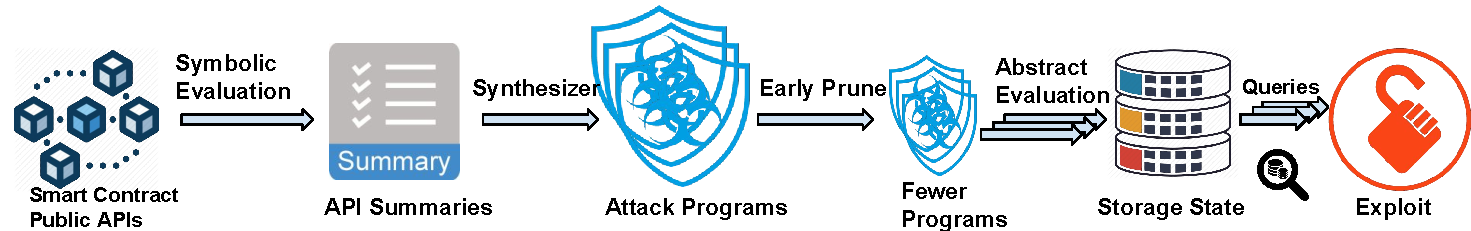
\includegraphics[width=\textwidth]{overview-ex.pdf}
% \caption{Overview of \toolname}
% \label{fig:overview}
% \end{figure*}
In summary, this paper makes the following contributions:\looseness=-1
\begin{itemize}
% \item We formalize the problem of finding smart contracts vulnerabilities as the problem 
% of synthesizing an attack program, which allows us to precisely model all possible interactions provided by the public ABI
% of smart contracts.
% \item  We present a simple but general query language for describing common vulnerabilities over program states in smart contracts.
% \item We develop an efficient synthesis algorithm and symbolic reasoning system for precisely 
% synthesizing adversarial contracts that exploits vulnerabilities specifying by the queries.
% \item  We implement the proposed ideas in a  synthesis tool called \toolname and demonstrate its effectiveness on a large data set from the Ethereum blockchain.
\item We formalize the problem of exploit generation as a program synthesis problem 
and provide a query language for expressing common vulnerabilities in smart contracts as declarative
specifications (Section~\ref{sec:vul}).
\item We propose a new summary-based symbolic evaluation technique for smart contracts that significantly reduces the number of paths that \toolname has to execute symbolically (Section~\ref{sec:sum}).
\item We develop an efficient attack synthesizer based on the summary-based symbolic 
evaluation, which incorporates a novel combination of search space partitioning, parallel
symbolic execution, and early pruning based on the semantics of
candidate programs (Section~\ref{sec:parallel}).
\item We perform a systematic evaluation of \toolname on the entire data set
from \etherscan. Our experiments demonstrate the substantial benefits of our
technique and show that \toolname outperforms three state-of-the-art smart
contracts analyzers in terms of running time, precision, and soundness
(Section~\ref{sec:eval}).
\end{itemize}
